\documentclass[fontsize=25pt]{scrbook}
%\usepackage{xeCJK}
\usepackage{amsfonts}
\usepackage{amssymb}
\usepackage{amsmath}
\usepackage{bm}
\usepackage[dvipdfmx]{graphicx}
%\setCJKmainfont{SimSun}
\title{Instructions Manual for AwayBus App} 
\author{Kwame Ackah Bohulu}
\date{\today}
\begin{document}
\maketitle

\newpage
\begin{center}
\begin{figure}
		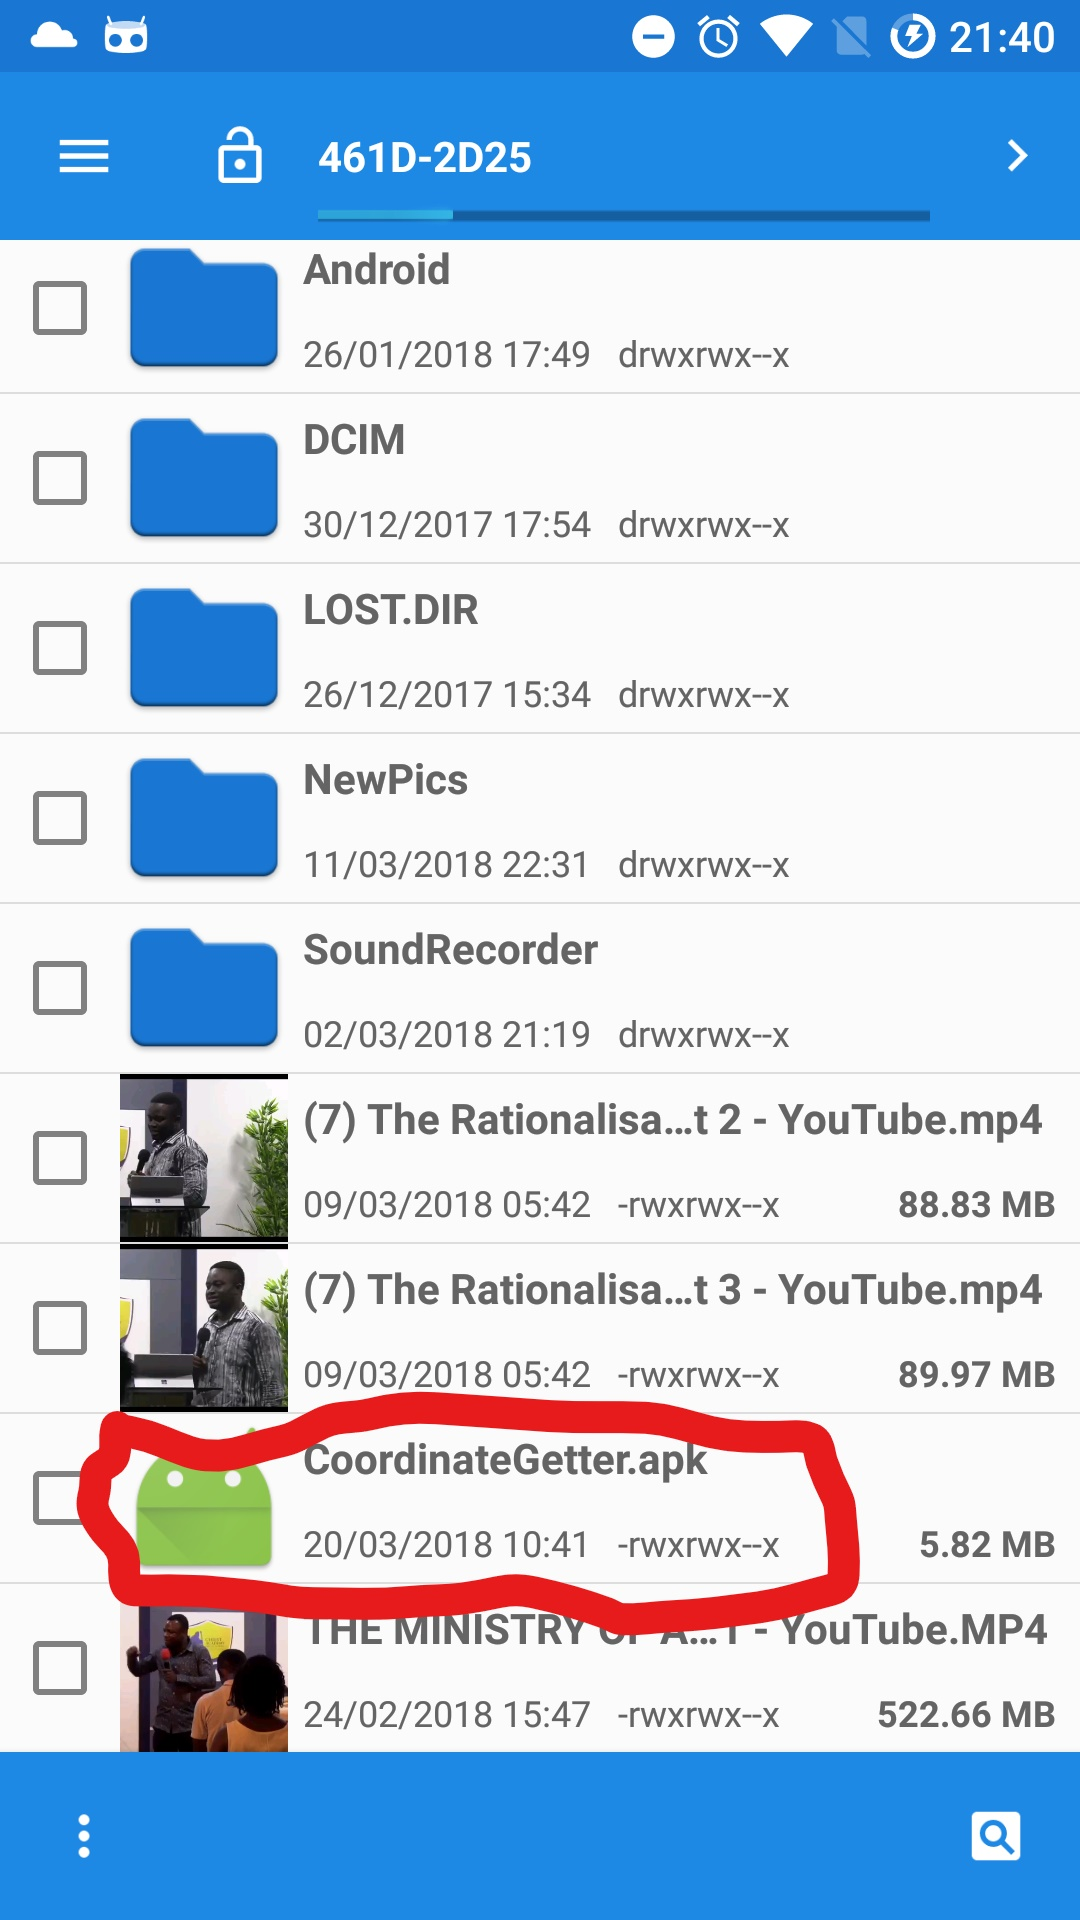
\includegraphics[height=10cm]{Screenshot_1_LI.jpg}
		
		\end{figure}
	\end{center}
Copy the app from your pc unto your device and tap on it to install. Please set your location settings to on.
\newpage
\begin{center}
\begin{figure}
		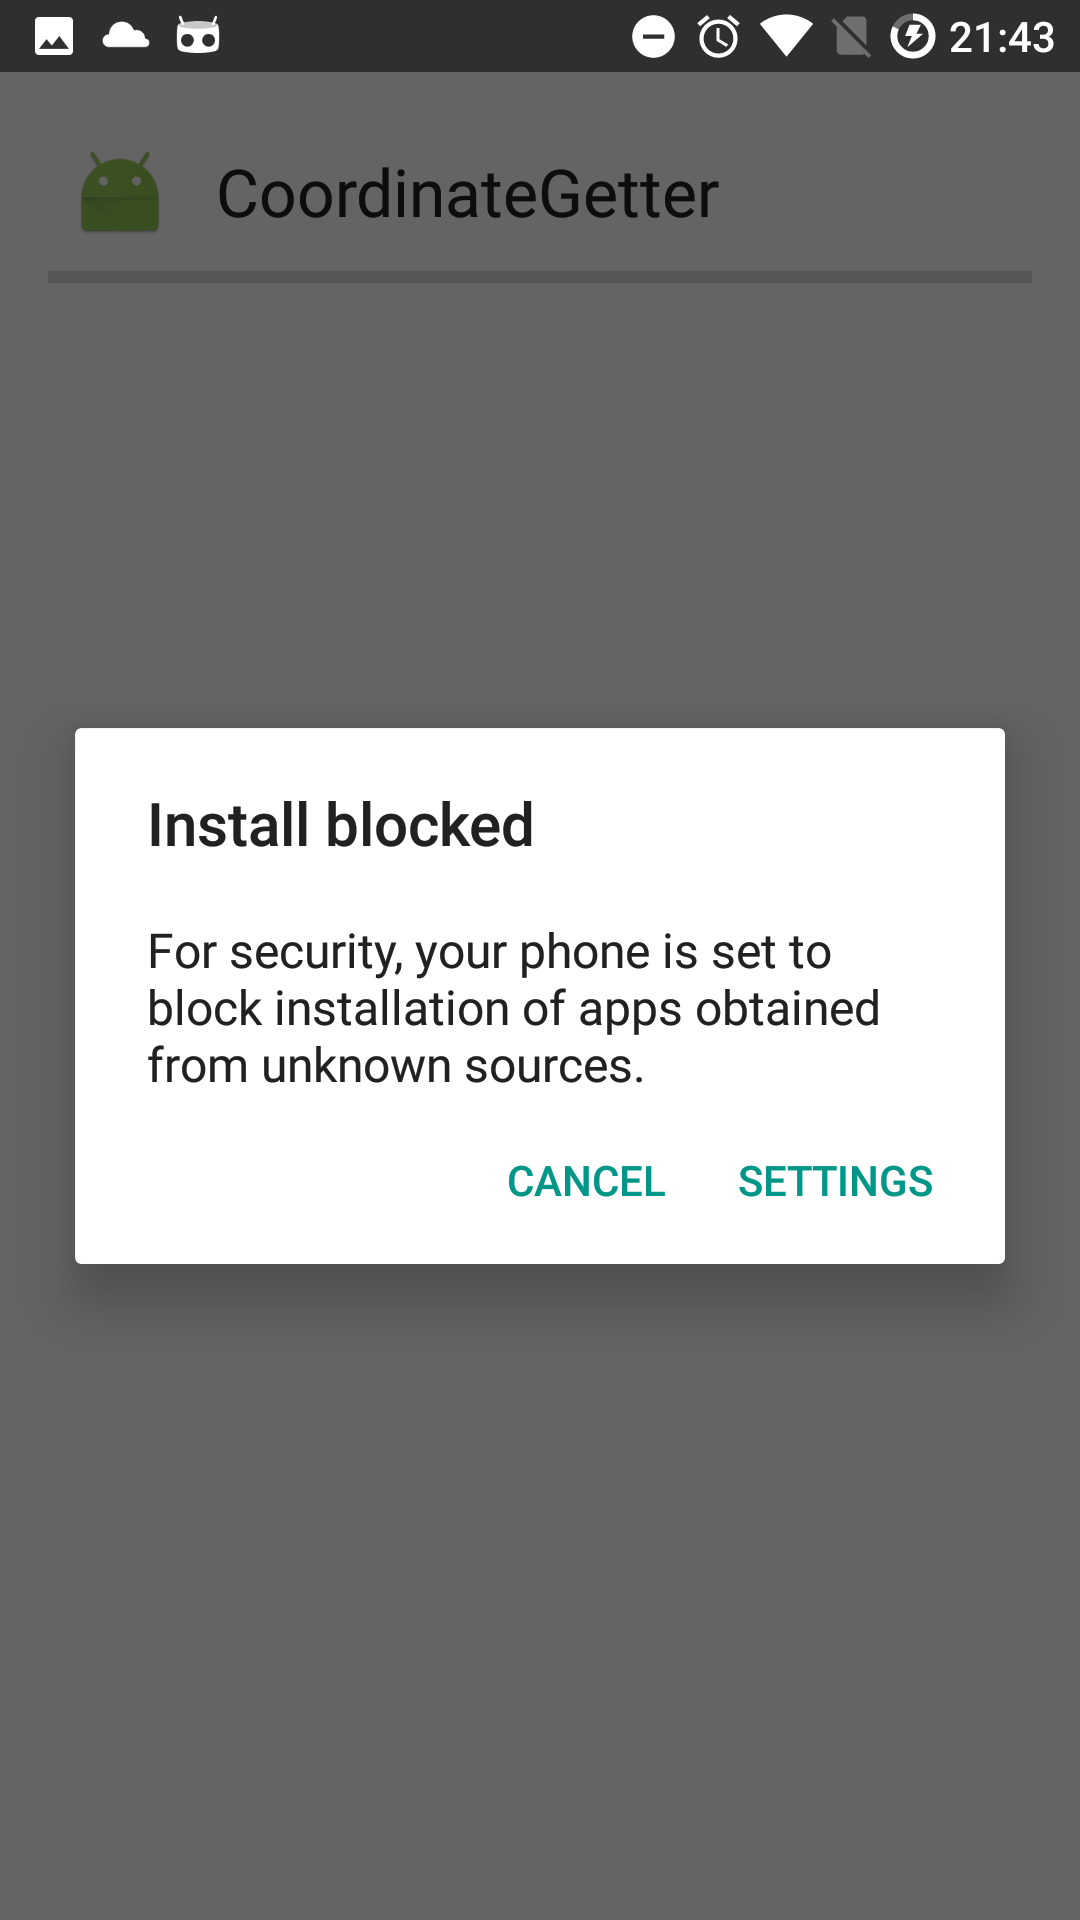
\includegraphics[height=10cm]{Screenshot_2.png}
		
		\end{figure}
	\end{center}
	In the case where you have not allowed installation from unknown sources,
	this popup appears. Click on settings to change the setting. Else go to page 6
	\newpage 
	\begin{center}
\begin{figure}
		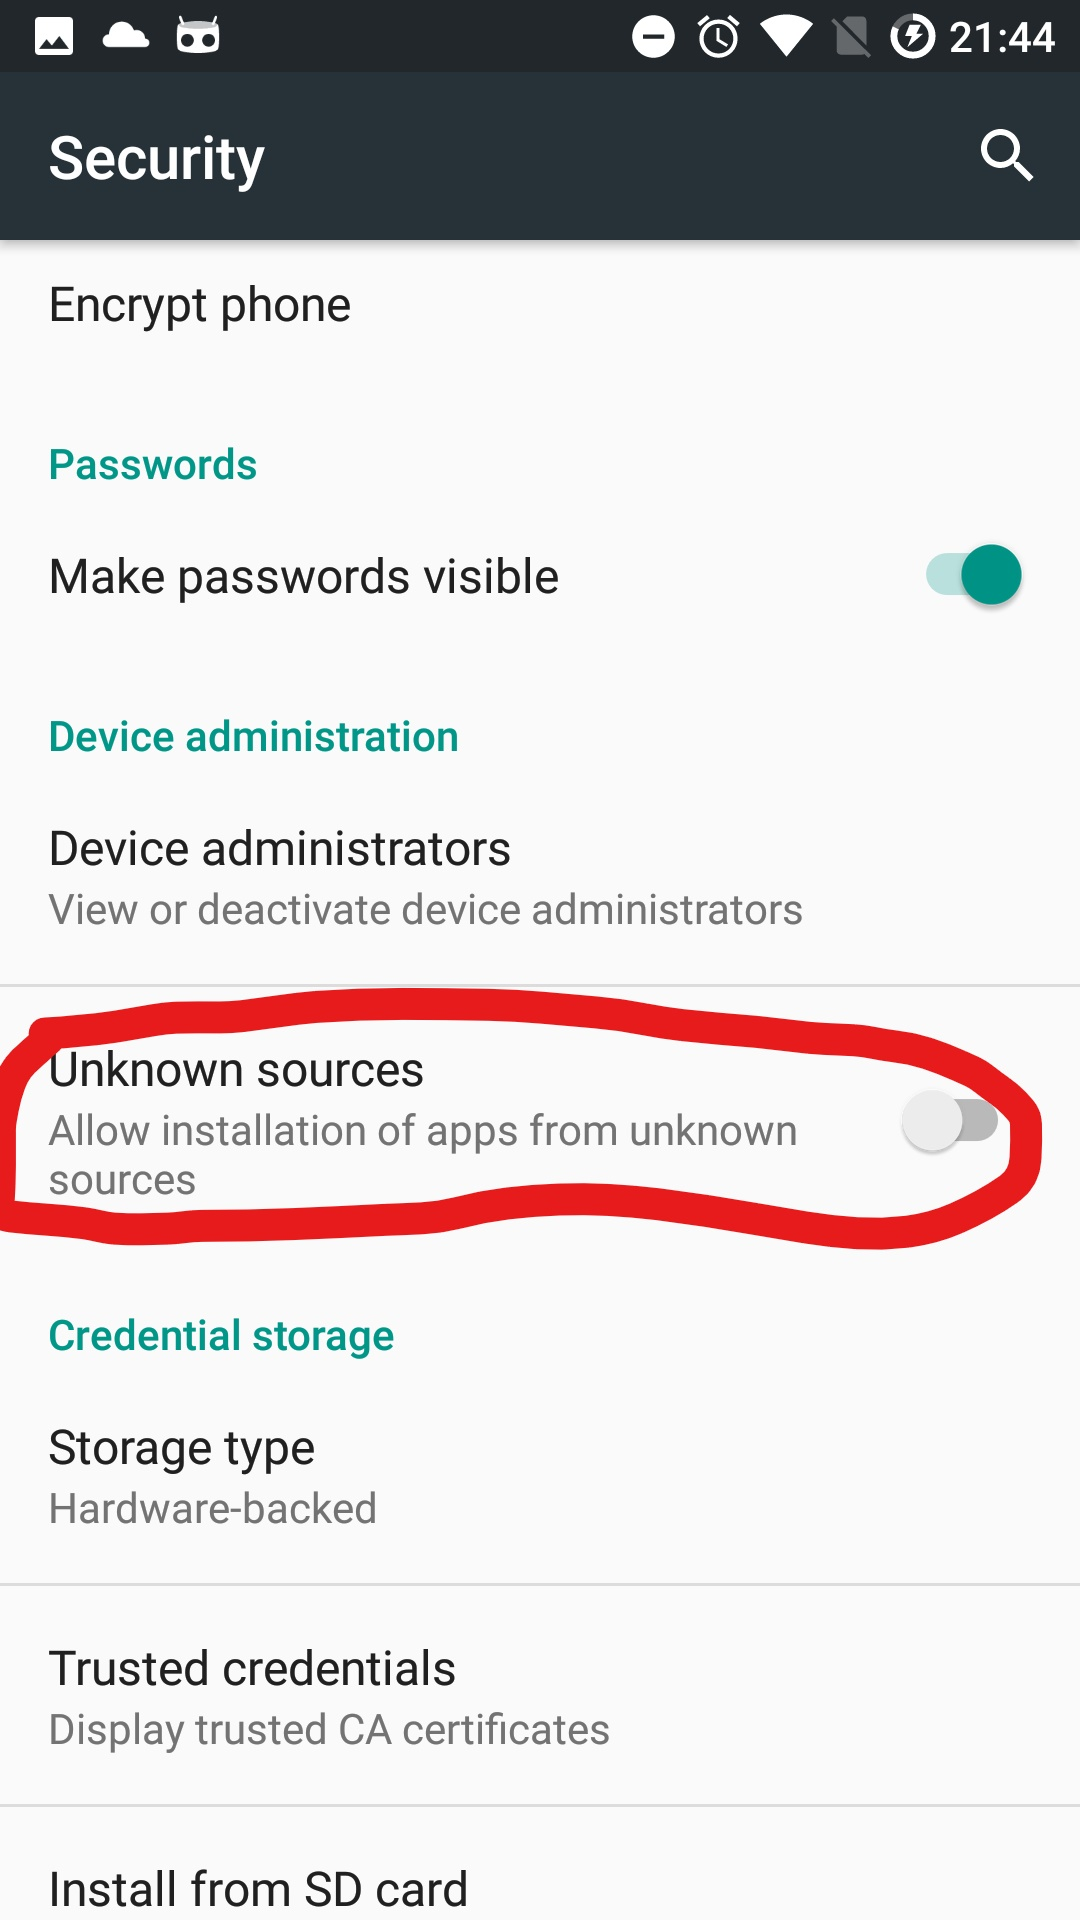
\includegraphics[height=10cm]{Screenshot_3_LI.jpg}
		
		\end{figure}
	\end{center}
	Click to allow installation from unknown sources
	\newpage
	
	\begin{center}
\begin{figure}
		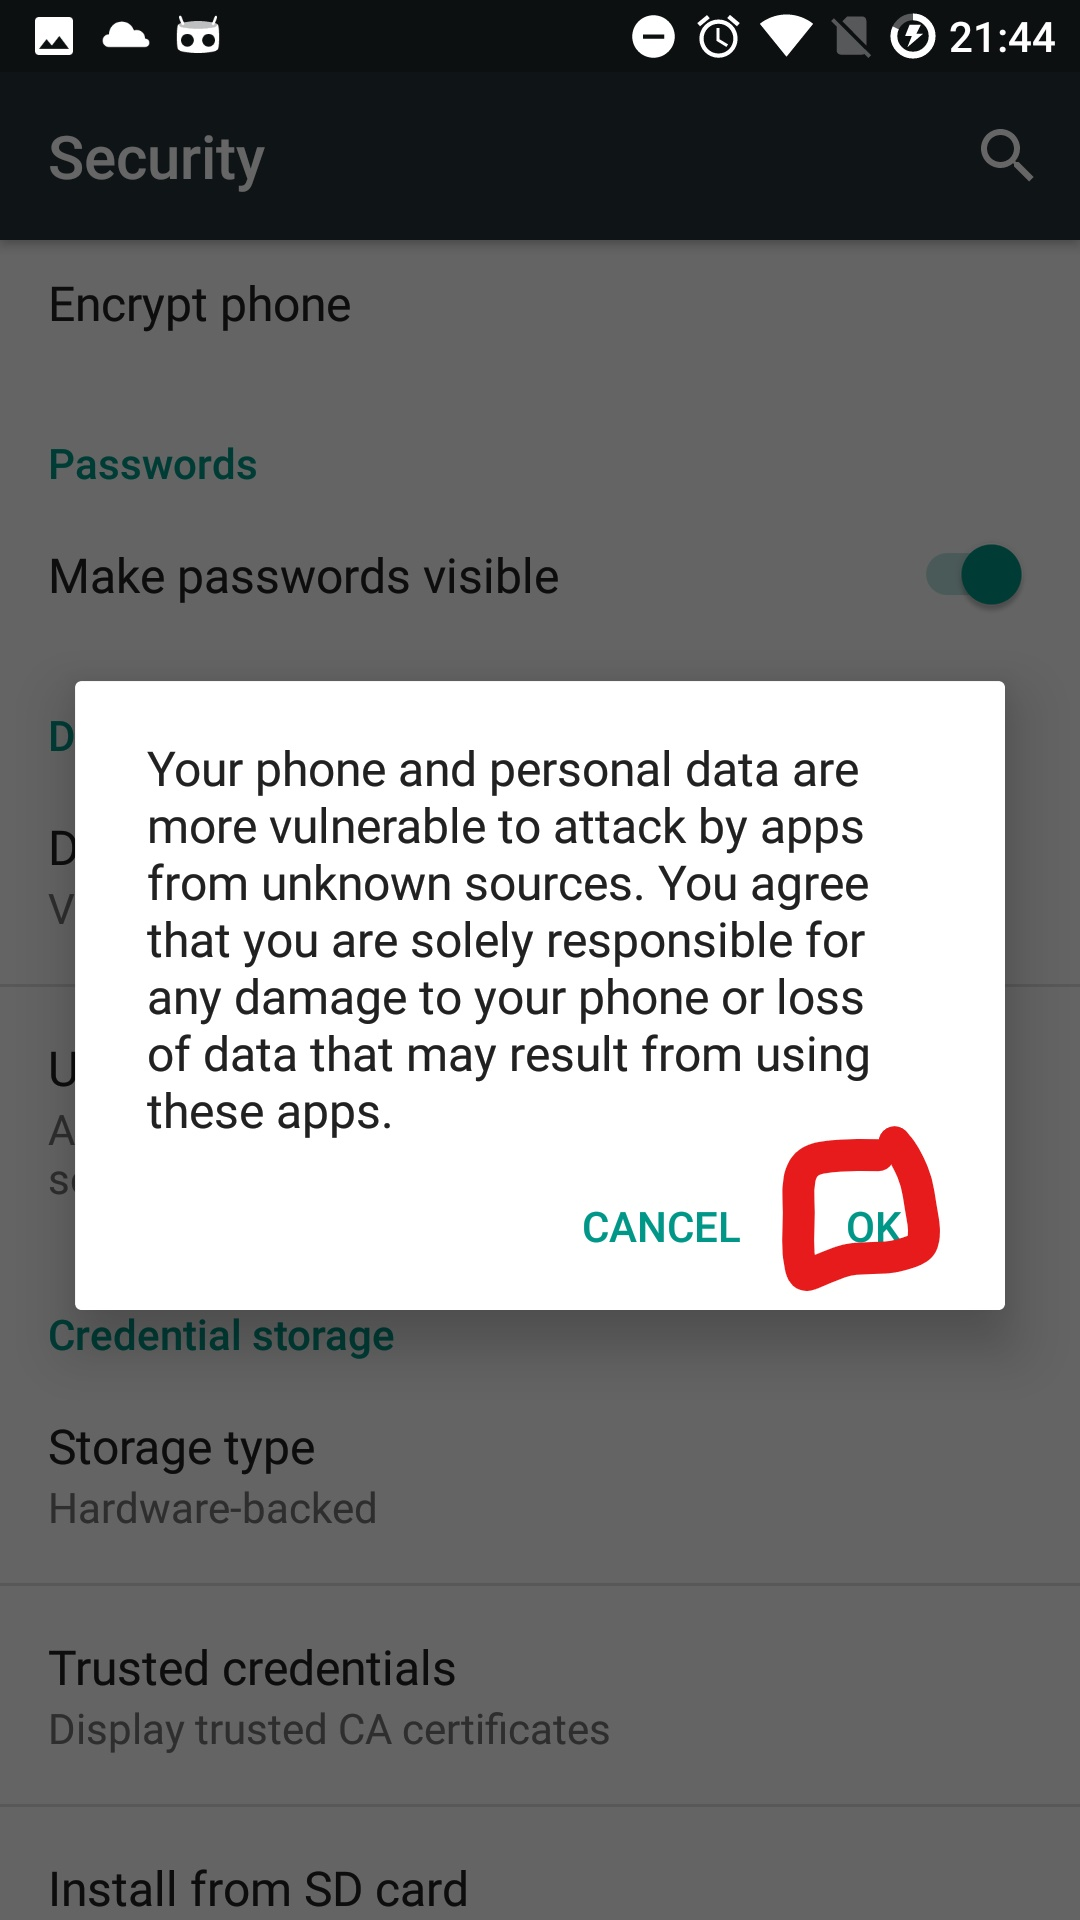
\includegraphics[height=10cm]{Screenshot_4_LI.jpg}
		
		\end{figure}
	\end{center}
	Click ok. Don't worry about the security part. My app is not a virus. Haha
	.Once complete, return to the location you copied the app to and try to install it again.
	
	\newpage
	\begin{center}
\begin{figure}
		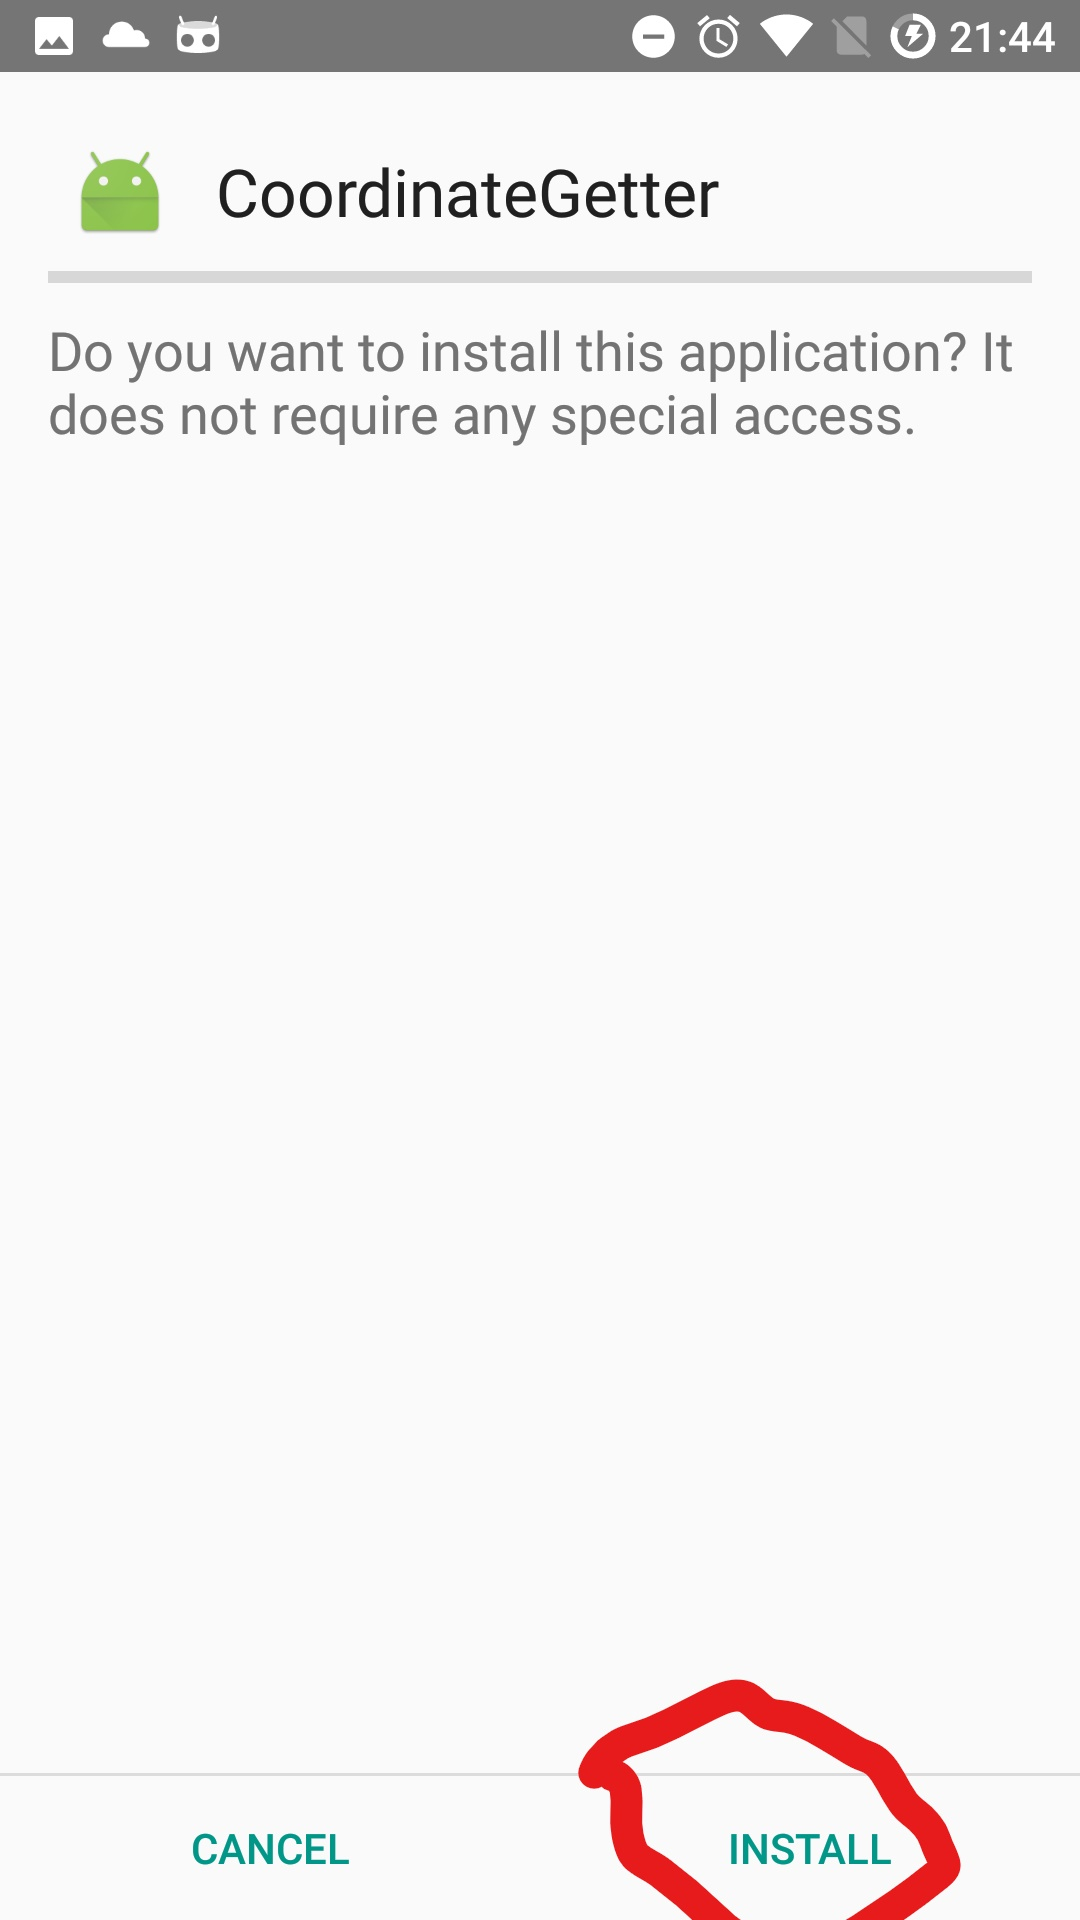
\includegraphics[height=10cm]{Screenshot_5_LI.jpg}
		
		\end{figure}
	
	Click on install to begin the installation process.

	\end{center}
	\newpage
	\begin{center}
\begin{figure}
		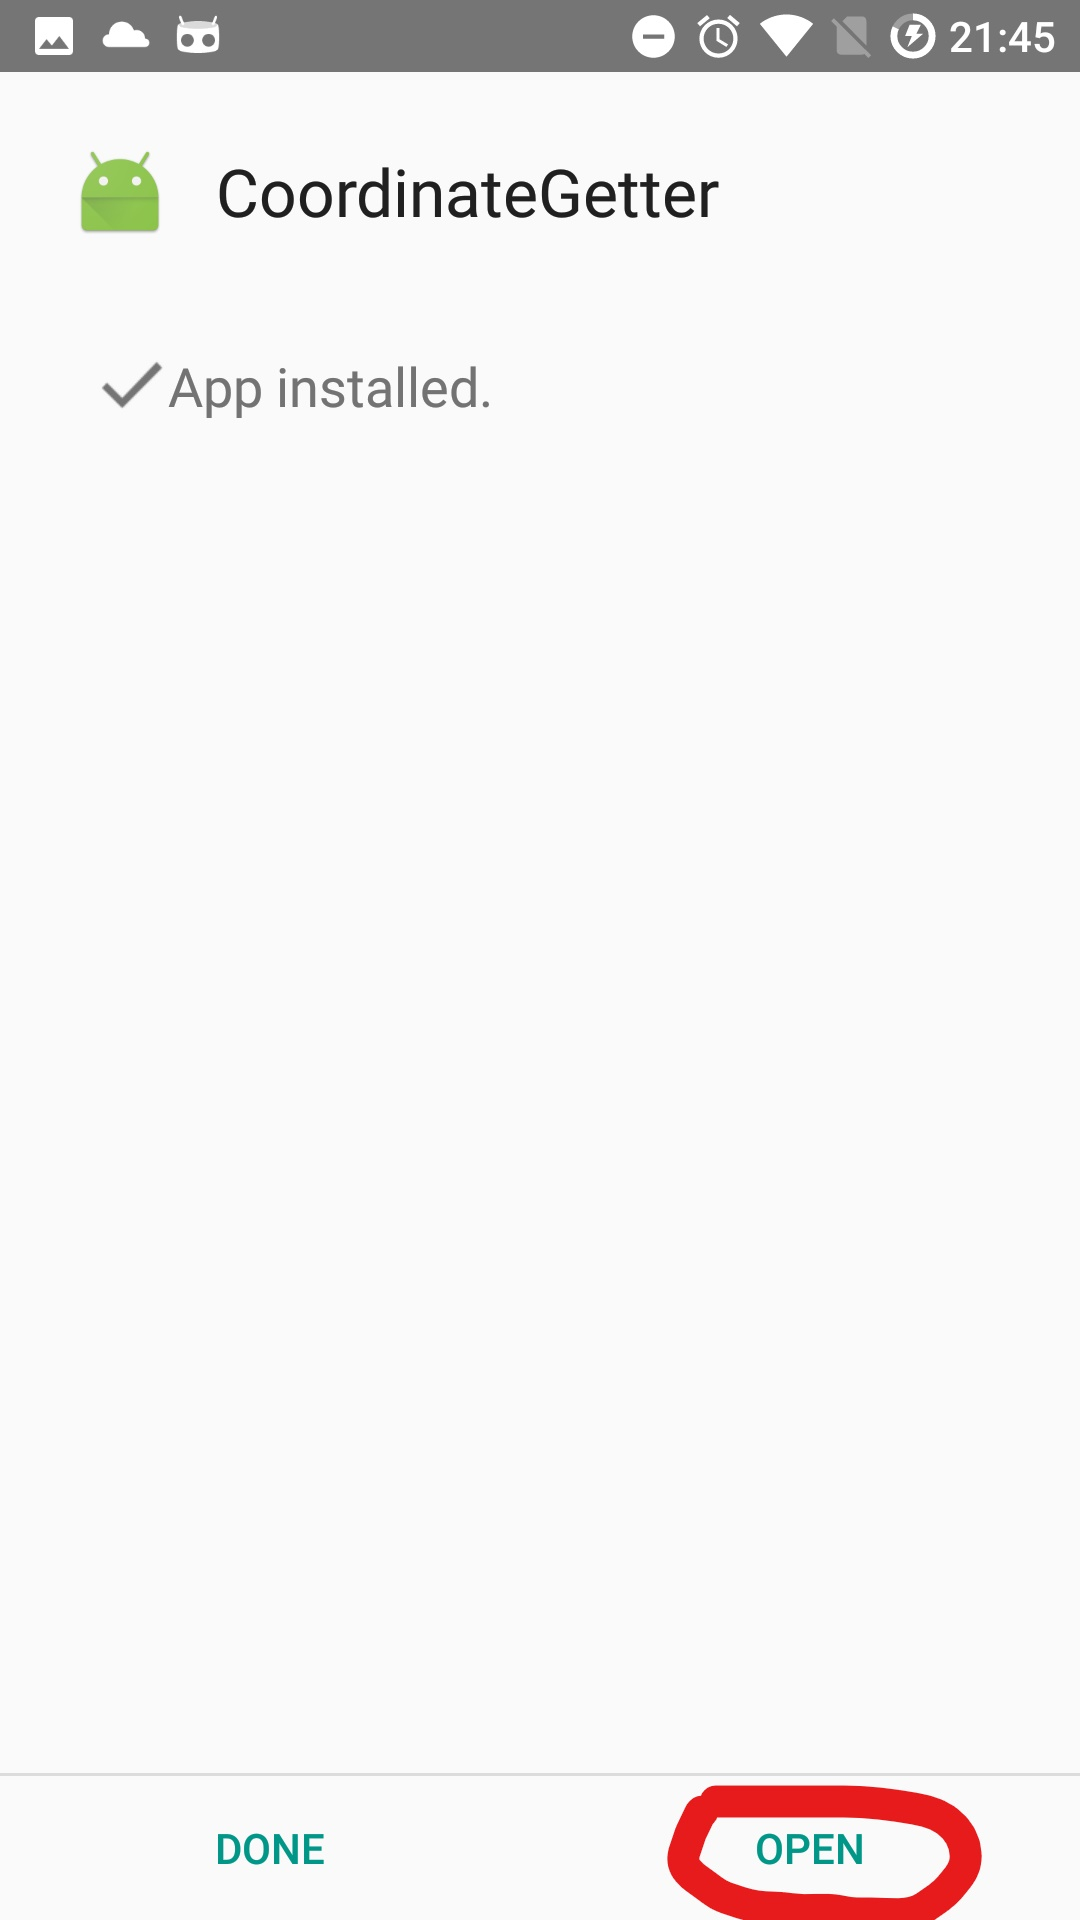
\includegraphics[height=10cm]{Screenshot_7_LI.jpg}
		
		\end{figure}
	\end{center}
	Once complete, click on the open button to start the app
	\newpage
	\begin{center}
\begin{figure}
		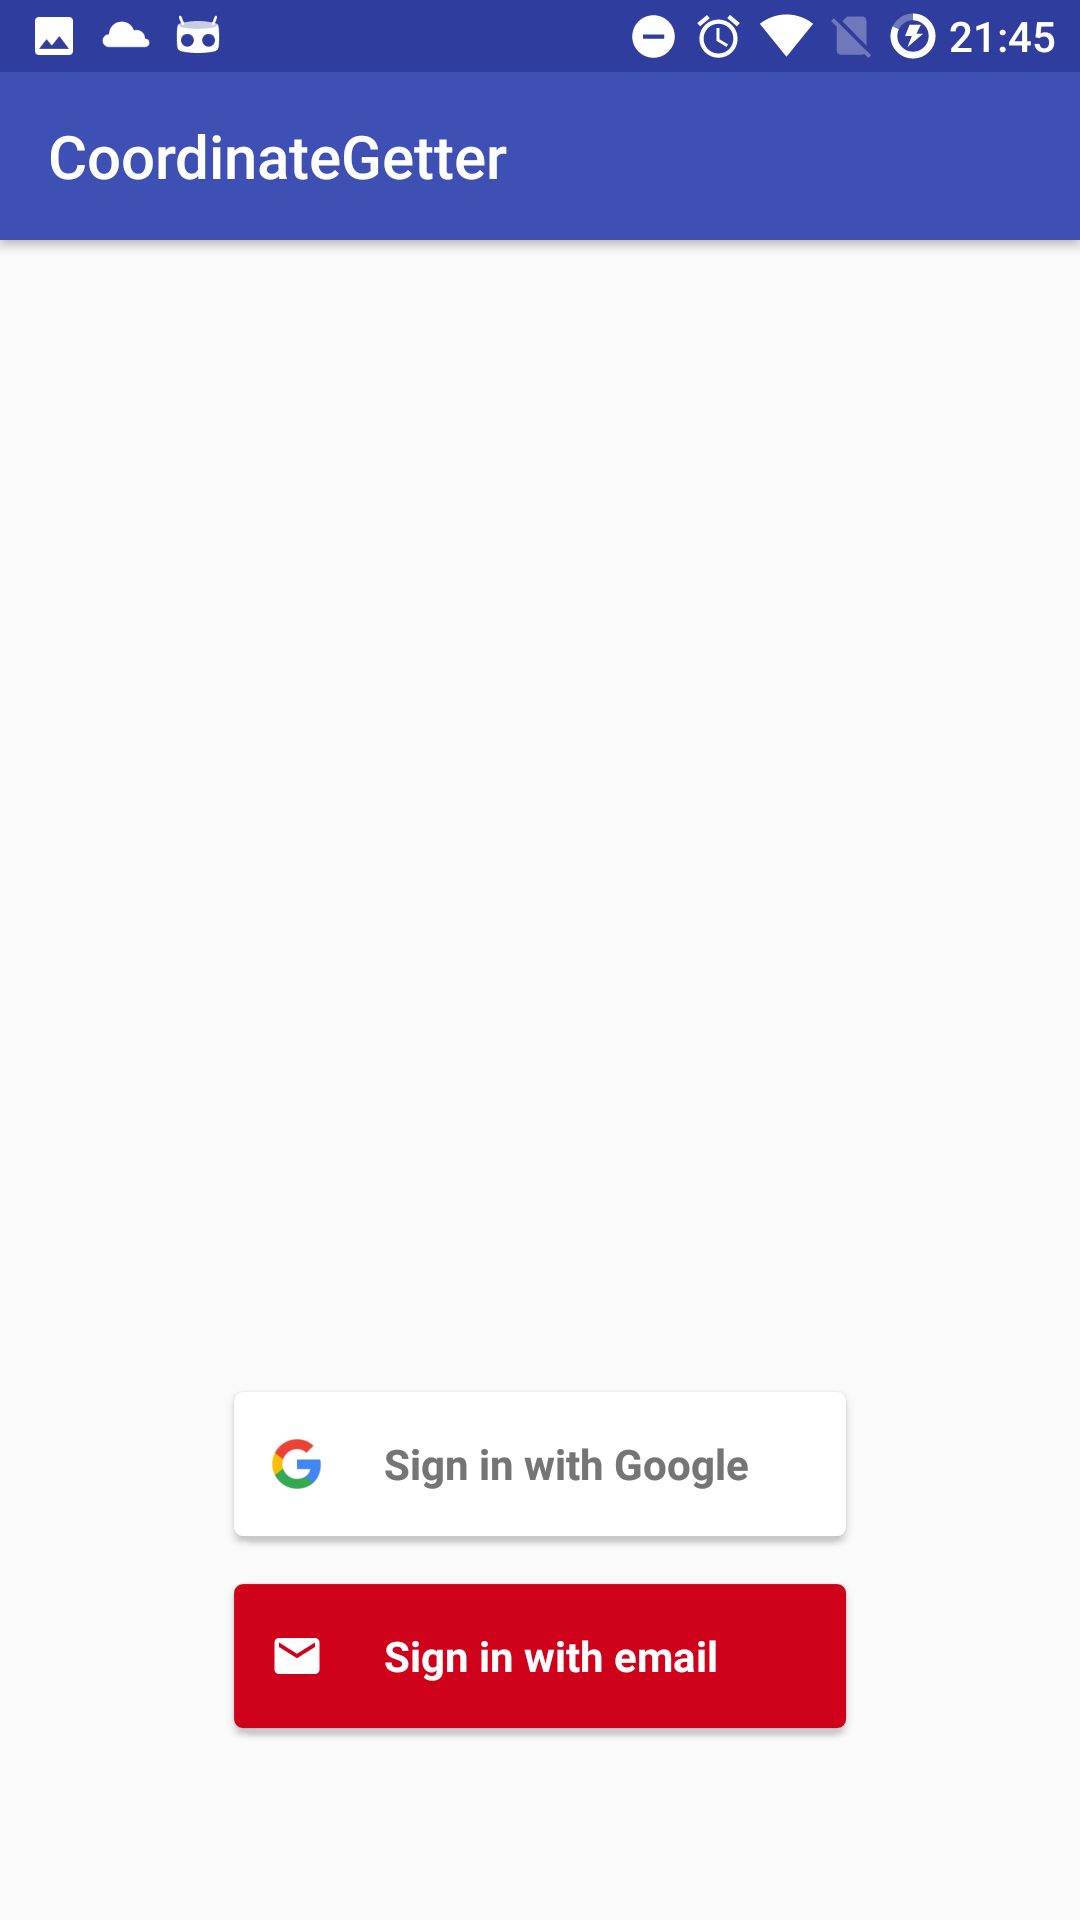
\includegraphics[height=10cm]{Screenshot_8.png}
		
		\end{figure}
	\end{center}
	Your email is required for authentication purposes. Please select the sign in method of your choice and fill in the form accordingly.
	\newpage
	\begin{center}
\begin{figure}
		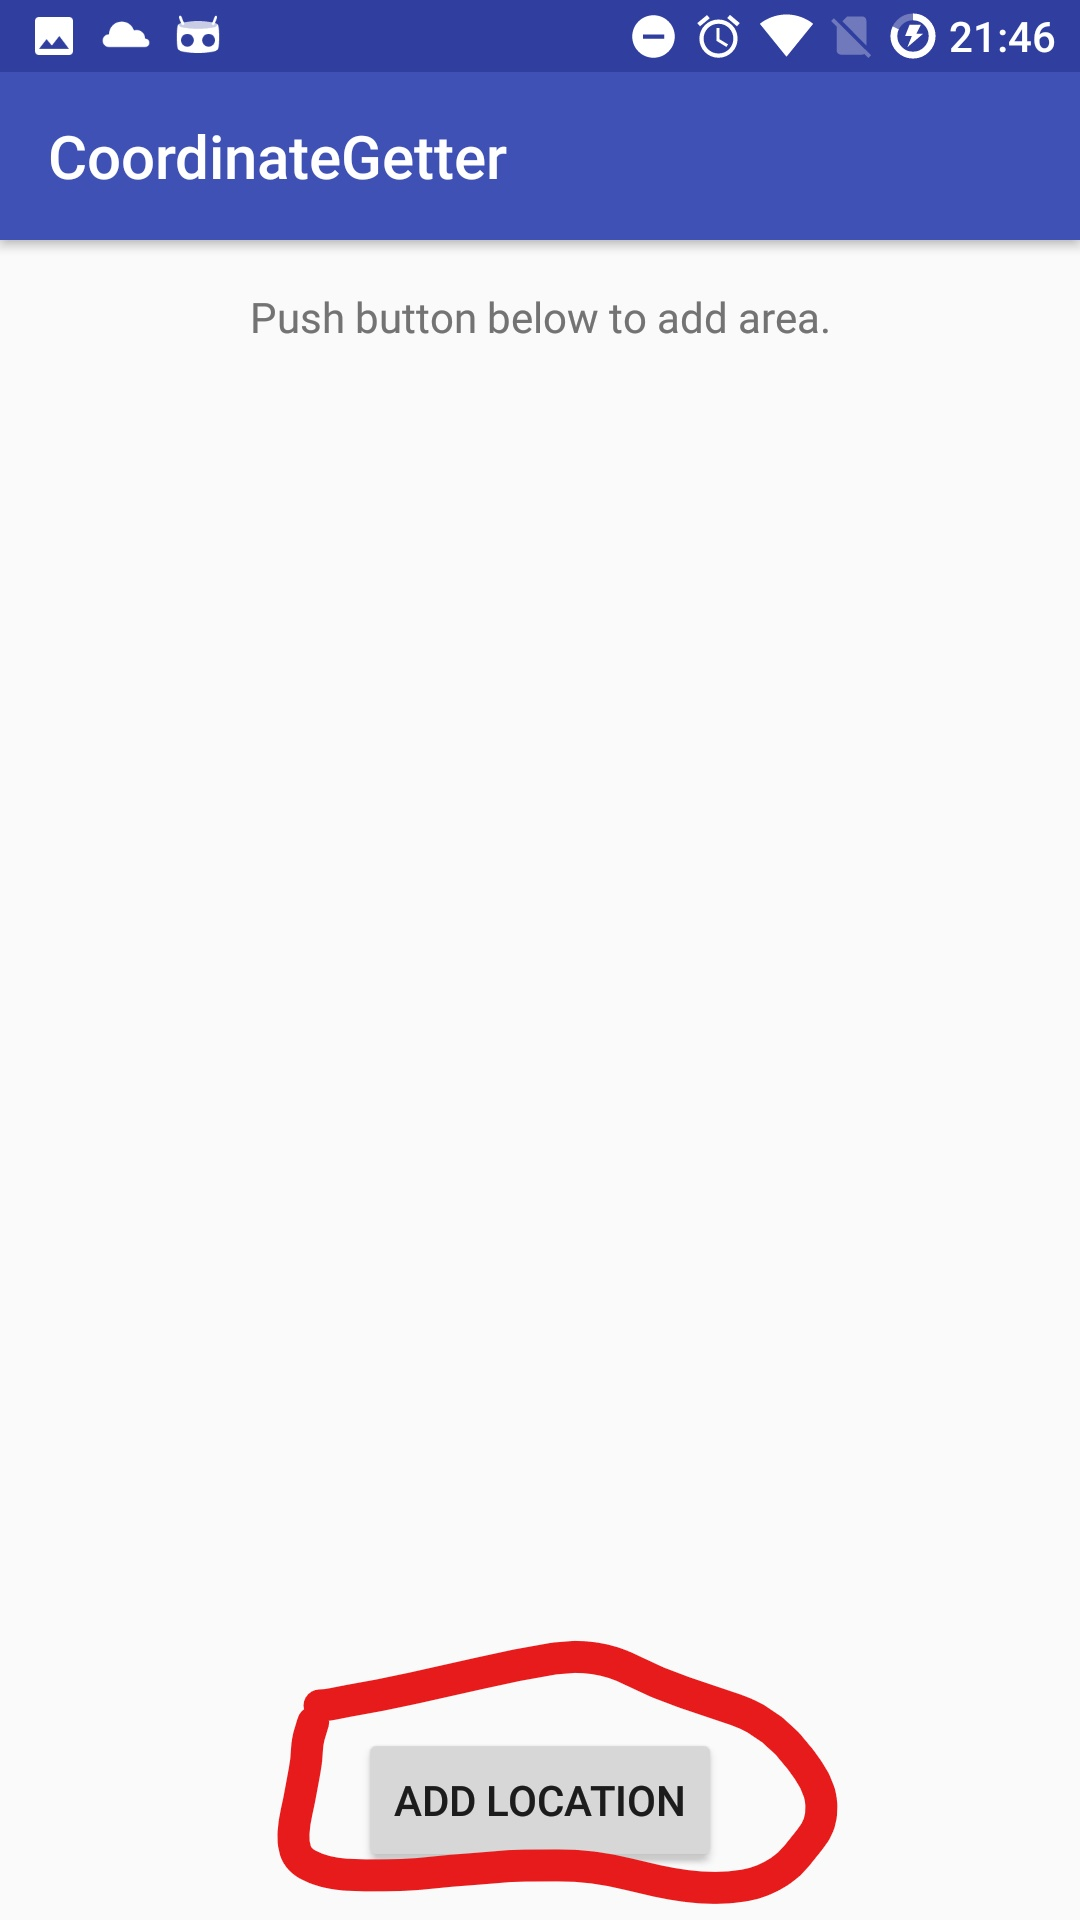
\includegraphics[height=10cm]{Screenshot_9_LI.jpg}
		
		\end{figure}
	\end{center}
	Click on the ``ADD LOCATION'' button to enter the Start Station name and the Destination Station Name. This denotes the beginning and end of the route taken by the bus.
	
	
	\newpage
	\begin{center}
\begin{figure}
		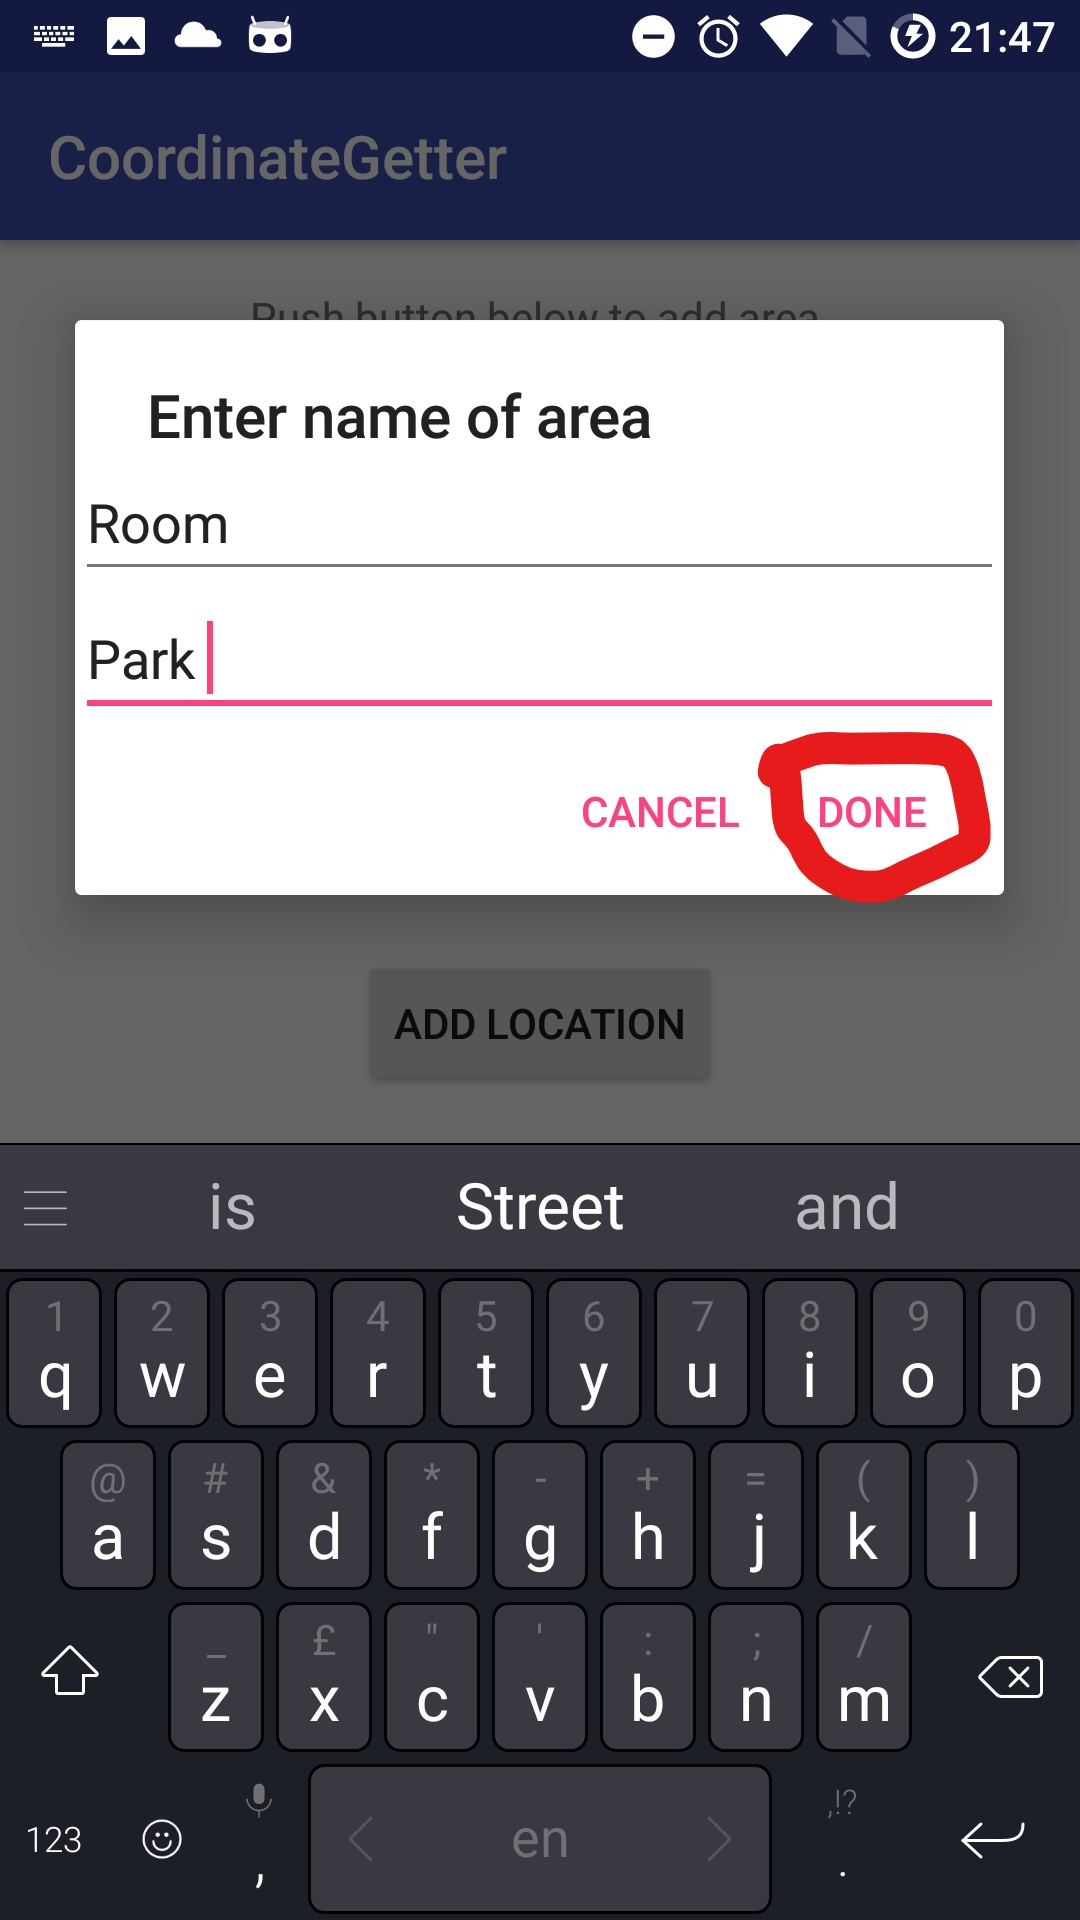
\includegraphics[height=10cm]{Screenshot_11_LI.jpg}
		
		\end{figure}
	\end{center}
	Please be sure to begin the name of each entry with a capital letter. Also make sure that the name selected is at least 4 characters long and does not include spaces.
	\newpage
	\begin{center}
\begin{figure}
		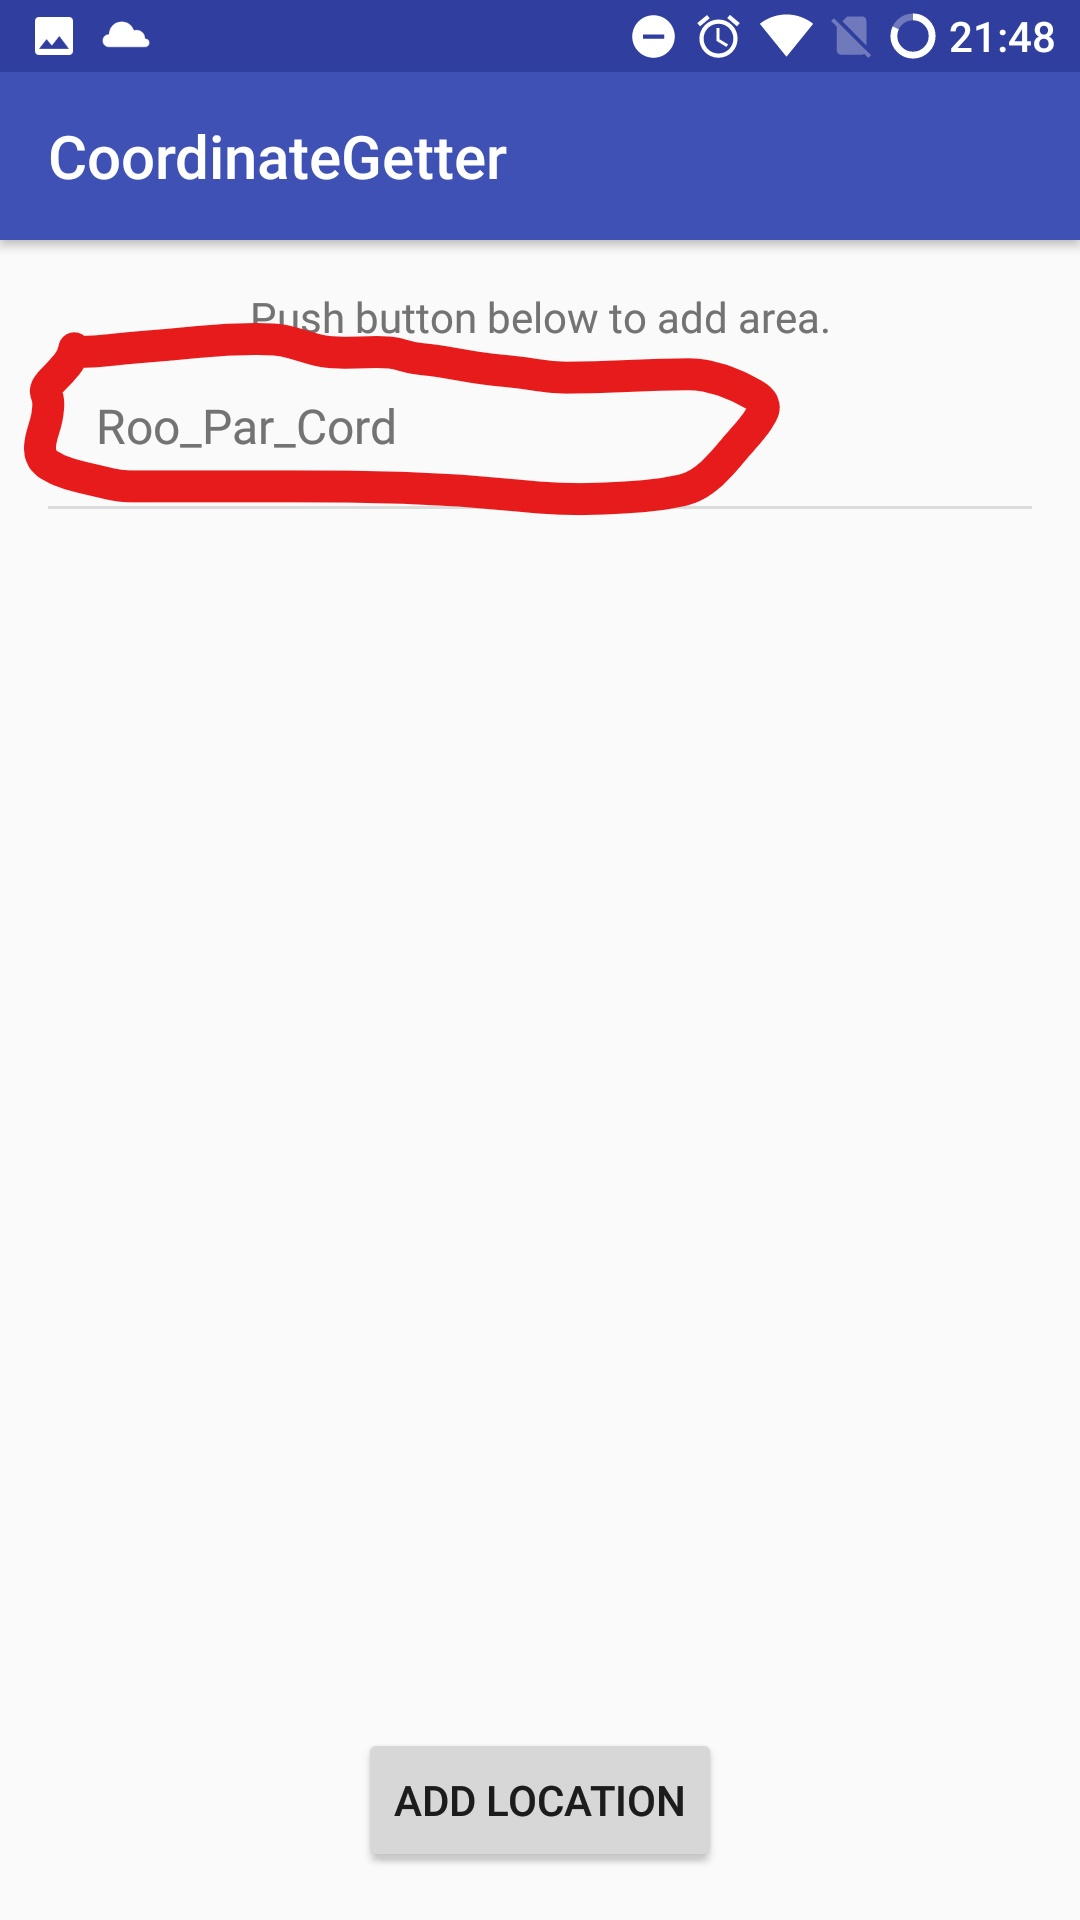
\includegraphics[height=10cm]{Screenshot_12_LI.jpg}
		
		\end{figure}
	\end{center}
	Click on the newly created area name to add bus stop name and GPS location information. Before that please be sure that your GPS is turned on to avoid errors
	\newpage
	\begin{center}
\begin{figure}
		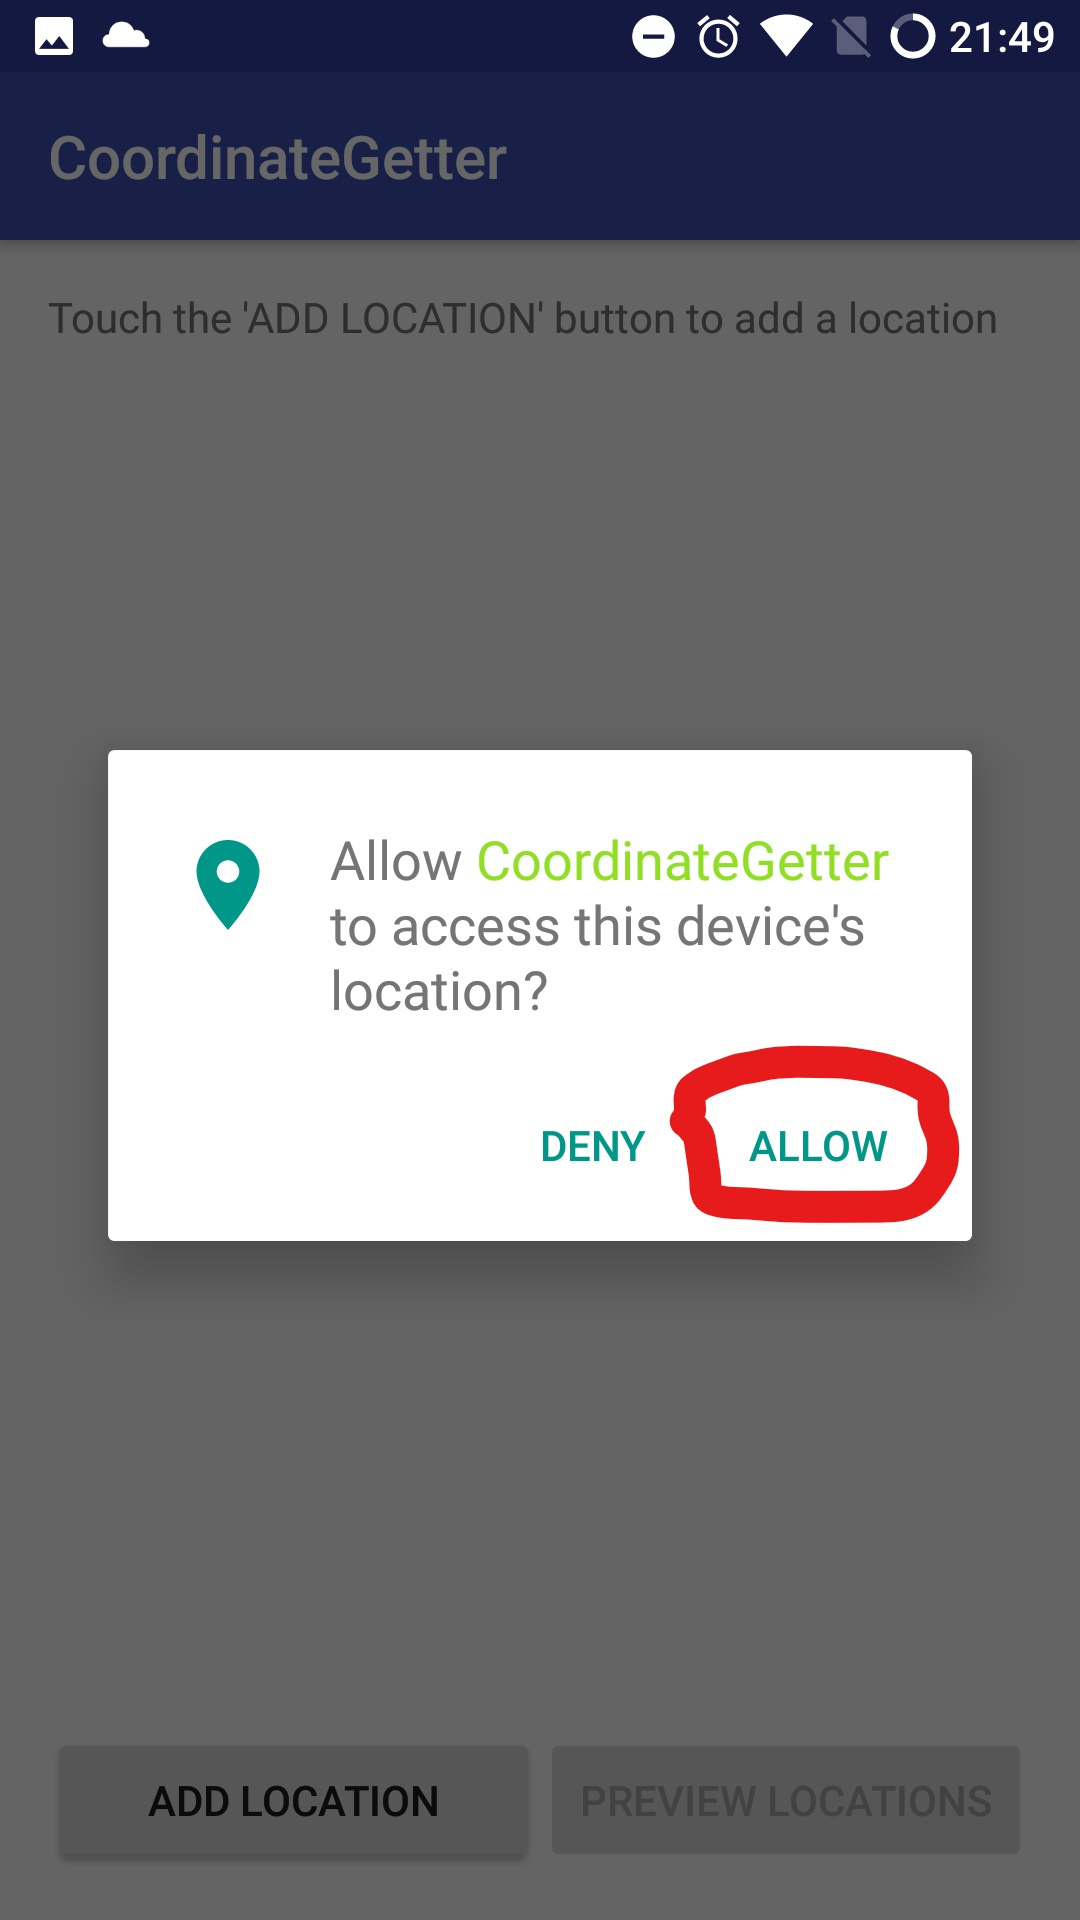
\includegraphics[height=10cm]{Screenshot_13_LI.jpg}
		
		\end{figure}
	\end{center}
	Allow CoordinateGetter access your device location.
	\newpage
	\begin{center}
\begin{figure}
		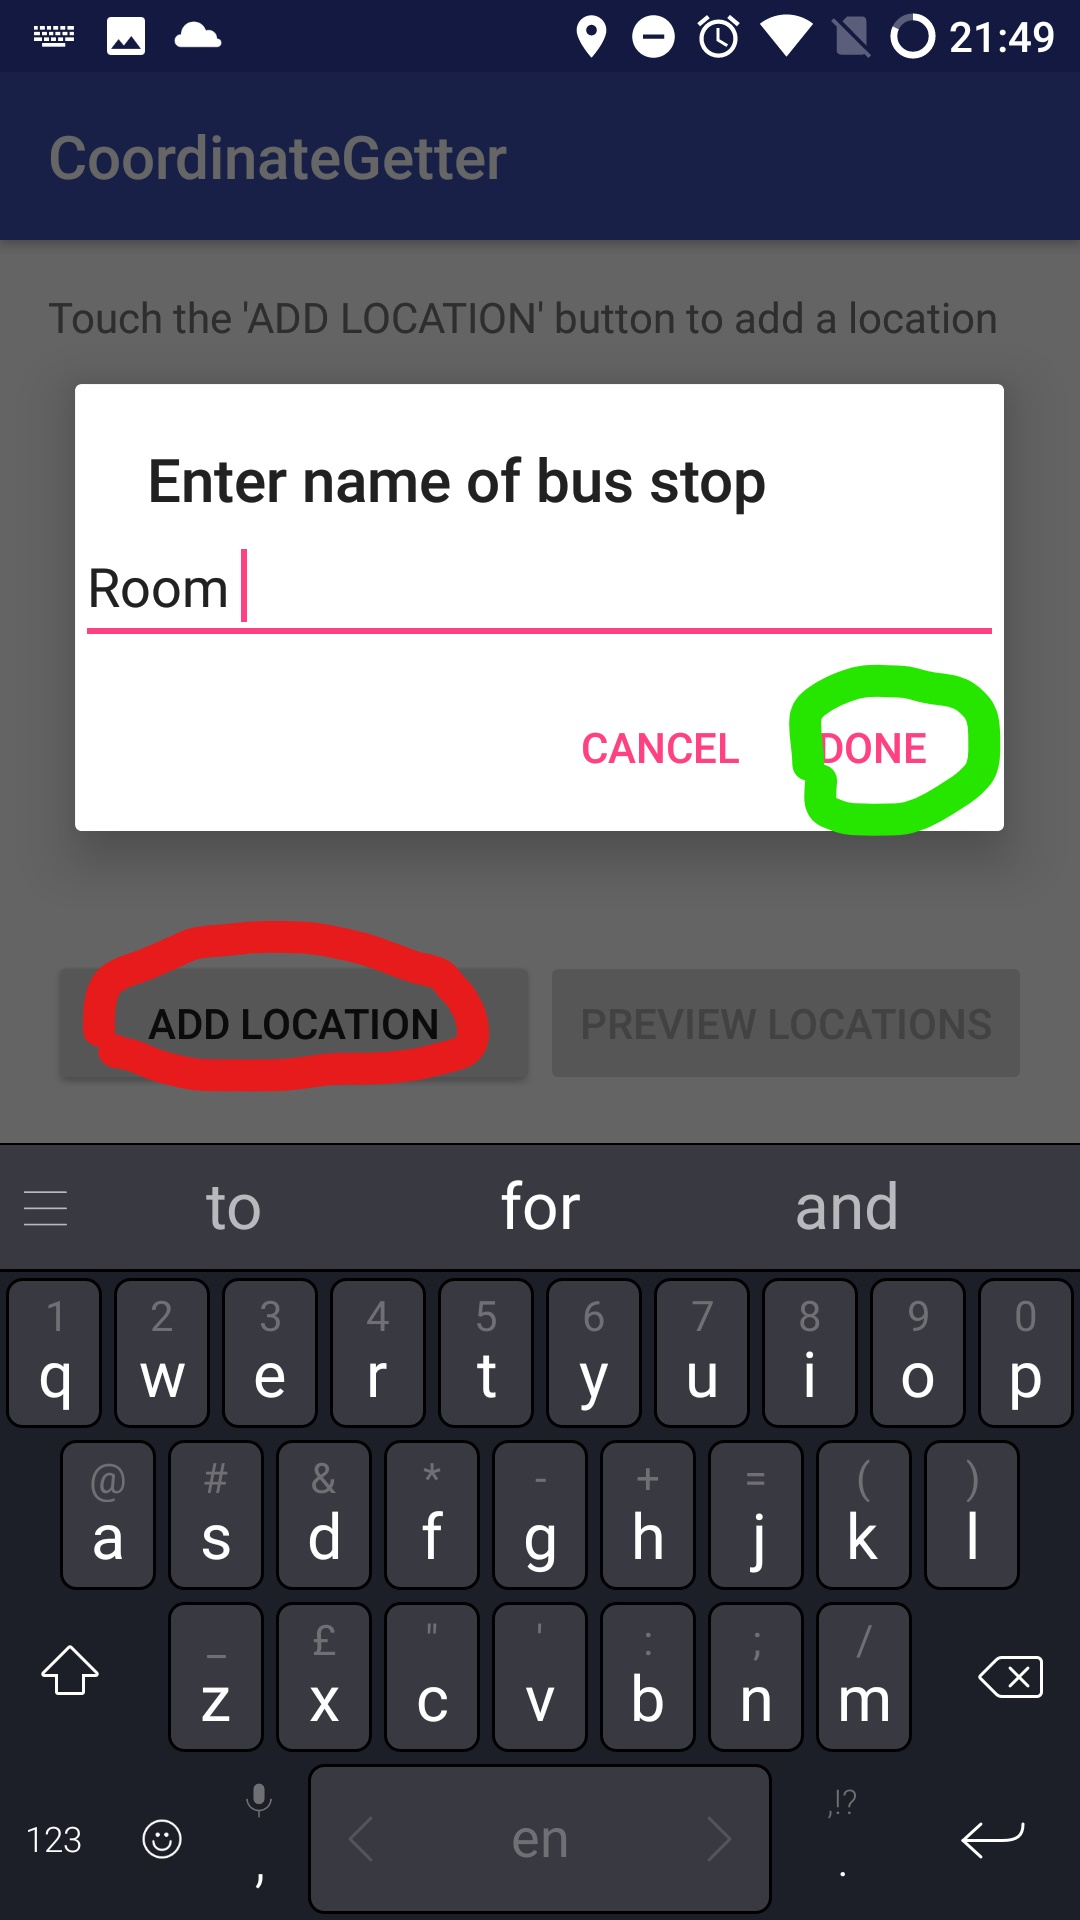
\includegraphics[height=10cm]{Screenshot_14_LI.jpg}
		
		\end{figure}
	\end{center}
	Once you get to the bus stop of interest, click on the ``ADD LOCATION'' circled in red to input the name of the bus stop. Click ``Done'' once the input is complete. Please be sure to begin all bus stop names with a capital letter.
	Repeat this for all other bus stops on that route.
	\newpage
	\begin{center}
\begin{figure}
		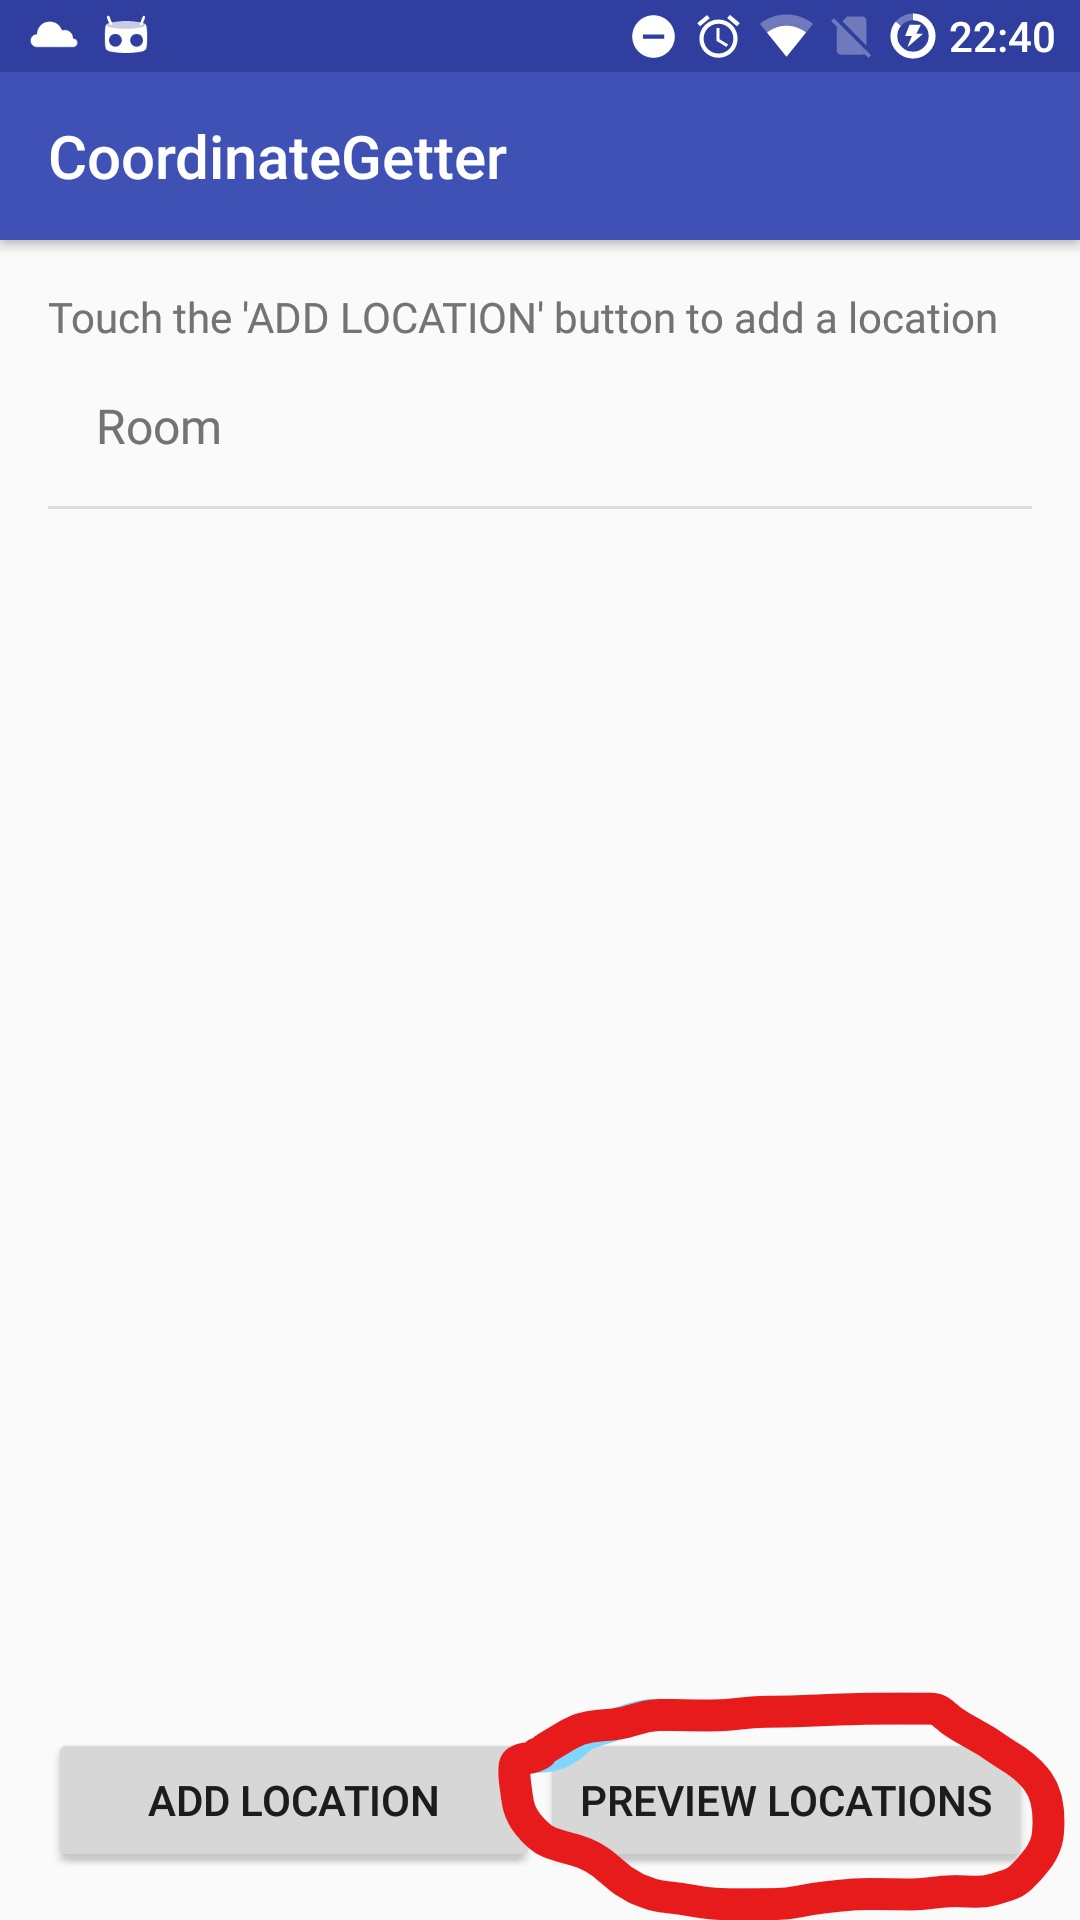
\includegraphics[height=10cm]{Screenshot_15_LI.jpg}
		
		\end{figure}
	\end{center}
	Once complete, click on the ``PREVIEW LOCATION'' button to view all bus stop names as well as the GPS coordinates.
	\newpage
	\begin{center}
\begin{figure}
		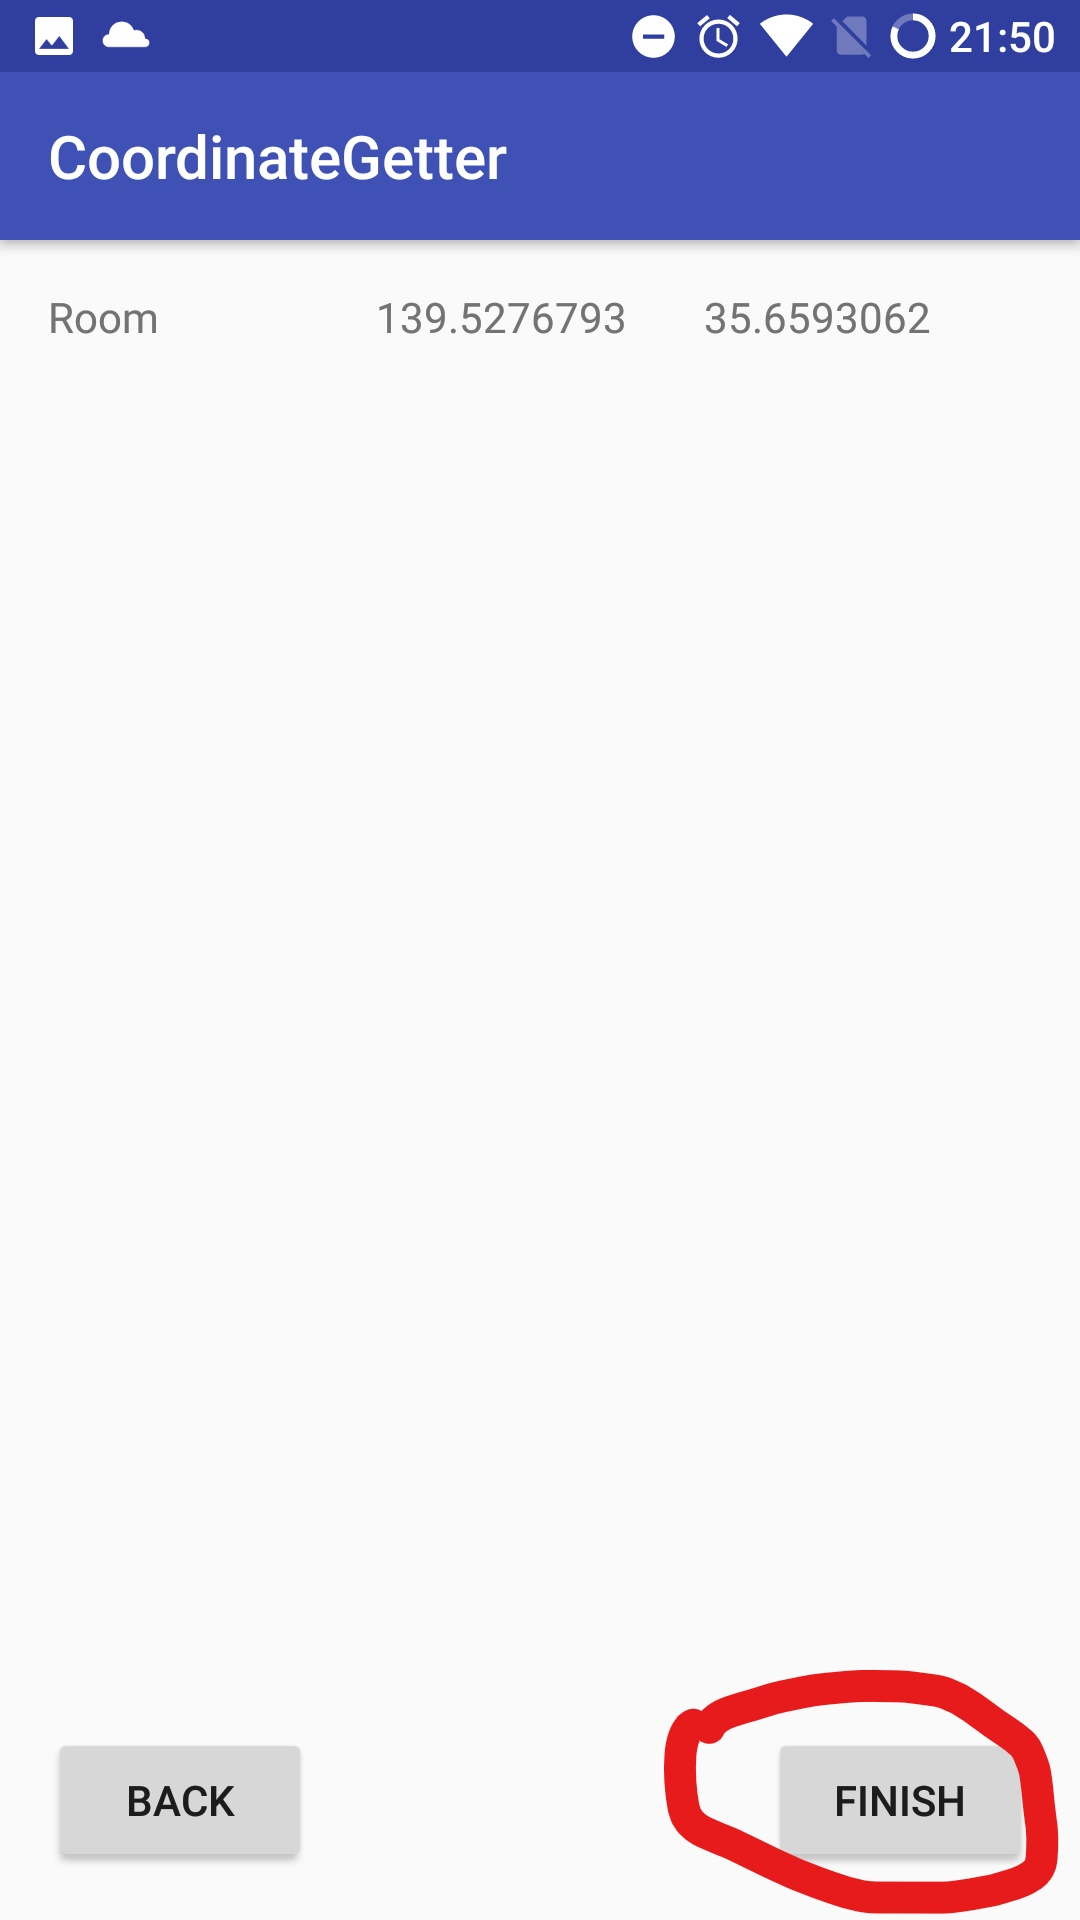
\includegraphics[height=10cm]{Screenshot_16_LI.jpg}
		\
		\end{figure}
	\end{center}
	If everything is satisfactory click on the finish botton to upload the infomation to the server.
	\begin{center}
\begin{figure}
		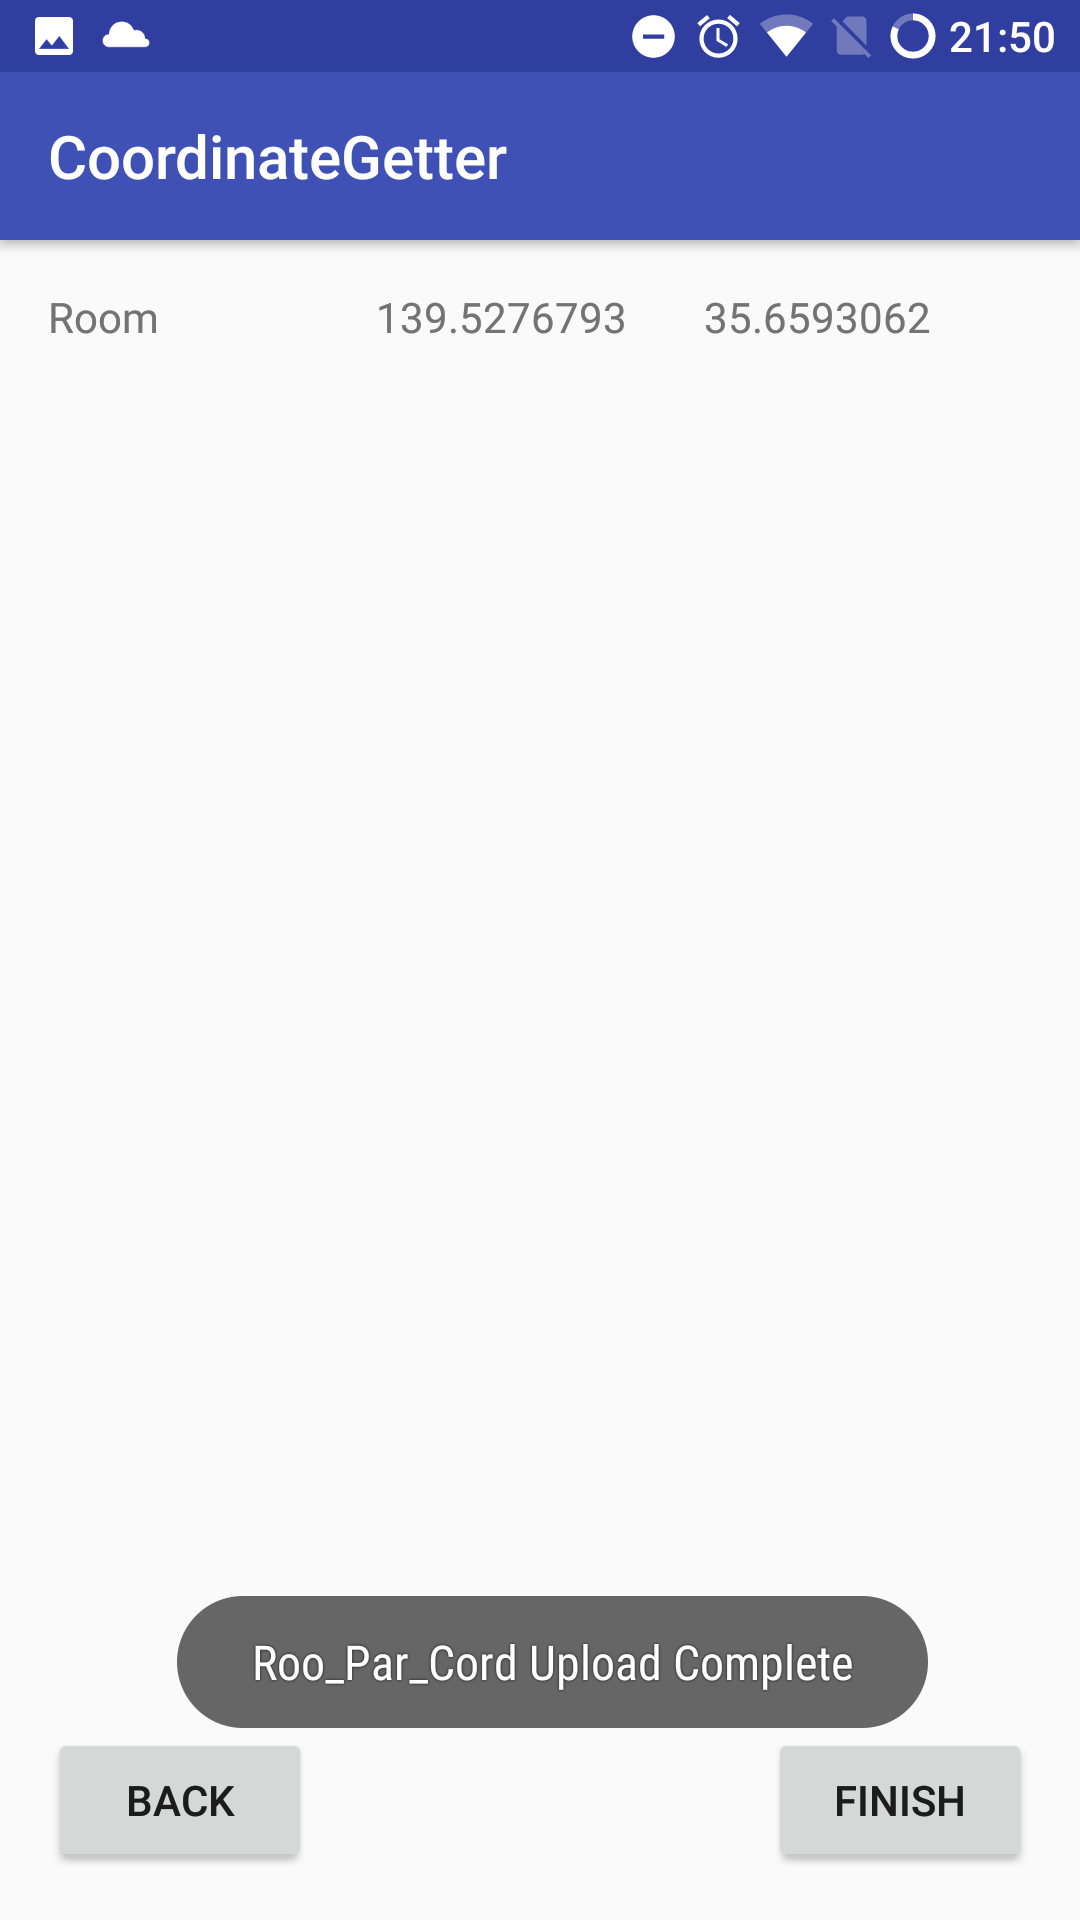
\includegraphics[height=10cm]{Screenshot_17.png}
		\end{figure}
	\end{center}
And you are done. Touch the back key many times to exit. Thanks for your help
\end{document}